\clearpage
\section{Dataset Statistics}
\label{appendix:dataset}
\begin{table}[h!]
\setlength{\abovecaptionskip}{-0.2cm}
\setlength{\belowcaptionskip}{-0cm}
% \footnotesize
\resizebox{0.48\textwidth}{!}{%
\begin{tabular}{lrrrrr}
\hline
Dataset & \# Users & \# Items & \# U--I & \# Concepts & \# C--C Pairs    \\ \hline
Course     & 34,235 & 4,322  & 89,565        & 5,131       & 227,515    \\
Movie & 608    & 7,354  & 49,738        & 12,503      & 8,402,493  \\
Book      & 92,971 & 70,695 & 409,616       & 58,492      & 15,889,953 \\ 
\hline
\end{tabular}
}
\caption{Statistics of the datasets used in our experiments. U--I: user--item interactions; C--C pairs: concept-concept pairs. }
\label{table:dataset}
\end{table}

Detailed dataset statistics are shown in Table~\ref{table:dataset}. Our Course dataset is sparser per user, validating observations that educational activities are hard to recommend without any side information. 
We follow the commonly-used annotation method \cite{liang2017recovering,pan2017prerequisite,gordon2016modeling} in inferring prerequisite relations: manually labeling a small number of concept pairs to train a logistic regression to label the rest. We annotated 300 pairs $(c_i,c_j)$ for each task with $+1$ if $c_i$ is $c_j$'s prerequisite, $-1$ if $c_j$ is $c_i$'s prerequisite, or 0 if no obvious dependency relation exists.  Of the 300 labeled samples $80\%=240$ are used for model training, and the remaining $20\%=60$ are held out for testing. 
The main purpose of this process is to \textit{de-noise} the PKL scores by considering three indicators, discussed in \S~\ref{sec:rq1}.

\section{Detailed Microscopic Case Study of Generated Prerequisite Graphs}
\label{appendix:micro}

As shown in Table~\ref{tab:pre-sample}, prerequisite linking in our other two datasets feels less intuitive, but is meaningful nonetheless. Taking selected concepts from our Movie dataset for the film \textit{'Harry Potter'} as an example, we see that the film is learned as a prerequisite for the knowledge concept \textit{'Fate of Human'}.  This means that the source IMDB and TMDB documents mentioning \textit{'Harry Potter'} mention {\it 'Fate of Human'} but not vice versa, leading to a large PKL score, hence a prerequisite.  Casual inspection of the general Web confirms that {\it Harry Potter} is a foil for subsequent discussions about fate and free will, which makes sense.  While the prerequisite does not constitute a strictly sequential viewing order among {\it 'Harry Potter'} and other movies featuring fate and free will as a central theme, these soft constraints do model inspiration; in Books, people who have read \textit{'Alien'}-themed books may go on to choose similarly themed \textit{'Space Travel'} books, including \textit{'Star Trek'} novels.

We also find that prerequisite graphs have different structural properties. Course prerequisite graphs contain the richest dependency relations (i.e., longer average path and larger average node degree), while graphs for the Movie and Book datasets are sparser and shallower.
Our casual observation of the graphs also reveal that longer prerequisite paths correlate with more specific terms (e.g., {\it 'Voldemort'}), while the shorter paths refer to more general knowledge ({\it 'Love'}).
Both studies show consistency, in that movies and books have fewer dependencies on required prerequisites, as compared to the formal knowledge acquired in courses, but that such soft constraints still aid recommendation accuracy.

\section{The Role of Prerequisites in Recommendation}
\label{appendix:cases}
\subsection{What embedding size is most suited for prerequisite representation?} Here, we use Root Mean Squared Error (RMSE) and R Squared (R2) to measure the fidelity of the KEM prediction; that is, after encoding.  In the figure, KEM (Knowledge Encoding Module) refers to the results from knowledge encoding module alone (ablating recommendation), RM (Recommendation Module) refers to the training of recommendation target without constraints from KEM, and PDRS applies both sets of constraints.

Both plots in Figure~\ref{fig:klatent_dim} show a consistent trend: adding more latent dimensions improves knowledge representation and prerequisite capture.
Furthermore, the joint training in PDRS of both $\mathcal{L}_{PKL}$ and $\mathcal{L}_{Rec}$ shows a  slight but consistent benefit.  Both exhibit large improvements compared against optimizing RM alone. 
Seen this way, good prerequisite capture through PKL is its own reward, but has the free side effect of benefitting downstream recommendation as well.
\begin{figure}[h!]
% \setlength{\abovecaptionskip}{-0cm}
\setlength{\belowcaptionskip}{-0.2cm}
\centering
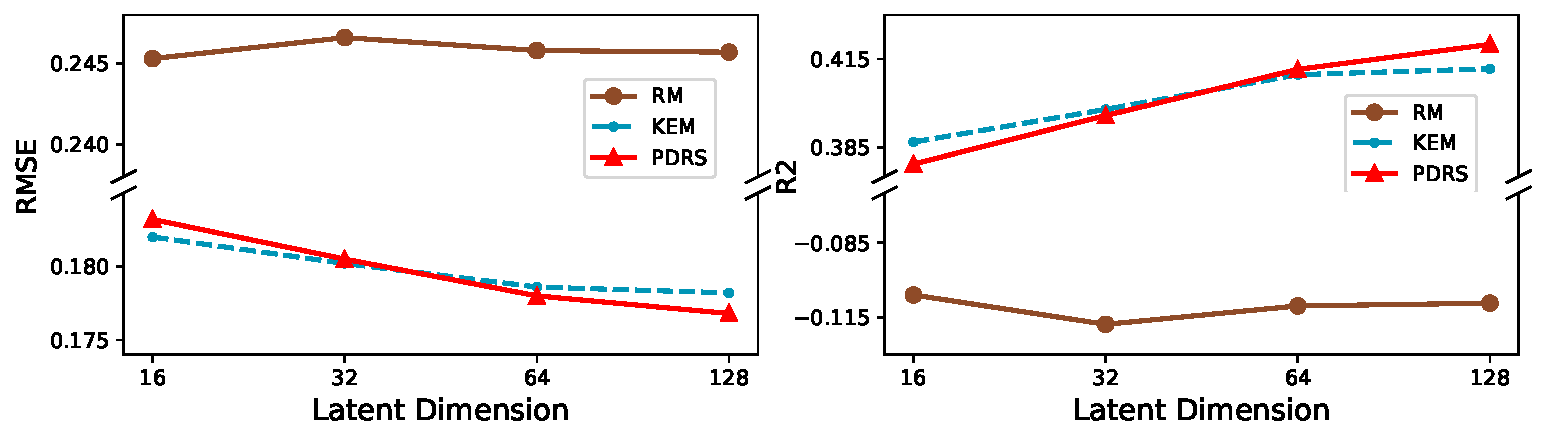
\includegraphics[width=0.7\linewidth]{res/kpl_encoding.pdf}
\caption{Effect of varying the dimensionality of the knowledge concept encoding (x-axes) on downstream recommendation performance (y-axes, as measured in (l) RMSE (lower better) and (r) R2 (higher better).}
\label{fig:klatent_dim}
\end{figure}

\subsection{Do prerequisites complement user--item interaction?}

Unlike collaborative filtering, prerequisites play a decisive and logical factor in driving users' sequential interactions with items.  While collaborative filtering may find quality recommendations, such recommendations may not account for the immediate needs of the user. 

Take the first row of Table~\ref{tab:micro} as in example of the role of such knowledge.  Here, the left portion of the table gives the input user's state of knowledge and the right portion shows the output recommendation from both the interaction-only BEM and our full PDRS.  
We see this user has handled basic office skills, and thus she may be interested in other related skills such as team work, or soft social skills, which may be recommended by collaborative filtering as is done in BEM.  But perhaps their priority is in building on existing credentials: here, \textit{'Microsoft Word'} can be seen as a more efficient means of  \textit{'text'} entry.

\begin{table*}[h!]
\footnotesize
\abovecaptionskip -0.5mm
\begin{tabular}{|l|ll|}
\hline
\textbf{User Context}  & \textbf{Model} & 
\textbf{First Recommended Item's Knowledge Concepts}  \\ 
\hline
\textbf{PriorK}: 'sort', '\underline{text}', 'ribbon', 'page orientation', 'manipulation' &    \textit{PDRS}  & 'read', 'document', 'page', 'undo', '\underline{microsoft word}'     \\ \cline{2-3}
\textbf{TargetK}: 'file', 'combo box', 'footnote', '\underline{layout}', 'form', 'controller' & \textit{BEM}   & 'team', 'development', 'plan', 'social response', 'application'    \\ 
 
\hline
\textbf{PriorK}: '\underline{muscle}', '\underline{tissues}', 'bone', 'mobile', 'neck' & 
    \textit{PDRS}  & 'autonomic nervous system', 'profile', '\underline{nervous system}', 'area'    \\ \cline{2-3}
\textbf{TargetK}: 'privacies', 'skill', 'certifier', 'participant' & \textit{BEM}   & 'compliance', 'requirement', 'response', 'investigation'     \\ 
  
\hline
\textbf{PriorK}: '\underline{protein}', '\underline{sugar}', 'food product', 'selection' & \textit{PDRS}  & 'bread', '\underline{baking}' \\ \cline{2-3}
\textbf{TargetK}: 'tour', 'participation', 'competition', 'visitor' & \textit{BEM}   & 'preventive act', 'report', 'unit'       \\ 
  
\hline
\textbf{PriorK}: 'conversation', 'spot', 'paper','detection' &  \textit{PDRS}  & '\underline{data analysis}', 'skill', 'sql', 'in demand', 'database'    \\ \cline{2-3}
\textbf{TargetK}: 'database', 'product', 'real world', 'code', '\underline{data feature}', 'universe' & \textit{BEM}   & 'facial', 'neck', 'eye', 'client', 'facial car'    \\ 
\hline
\end{tabular}
\caption{Course examples where PDRS behaves differently. \underline{Underlined concepts} are strongly induced by PKL.}
\label{tab:micro}
\end{table*}

\paragraph{Can prerequisite knowledge be derived from user--item interaction directly?} In short, yes, but much less effectively as we have done in PDRS.
To illustrate the fine-grained level of useful prerequisite knowledge captured (item or concept), we also benchmark PDRS with coarser, obvious prerequisites.   We build another item dependency graph directly from the interaction sequence order in our Course scenario.
We set an aggressive threshold, keeping only the top $\sim$250 item pairs satisfying a minimal number of occurrences and prerequisite strength.  We run these identified, salient prerequisites through BEM but find that performance suffers significantly, leading to a 3.6\% drop in performance. 
This finding direct attributes the power of the fine-grained prerequisite capture, and the effectiveness of PDRS in incorporating general features enhance the signal coming from sequential interaction histories.  


\section{Discussion: Is PDRS sensitive to hyperparameter setting?}

We examine how PDRS handles both prerequisite context and user/item encodings as the model complexity (in terms of hidden layers) is varied. As shown in Table~\ref{tab:pretrain}, models with or without pretraining both perform best with $L=4$.
Fewer layers are insufficient to learn the complex relationship between embeddings (especially for PDRS to learn the relation between knowledge embedding from both user and item), whereas larger numbers suggest overfitting. 

PDRS with pretraining achieves better performance with more hidden layers, but is worse than the case without pretraining, when number of layers is small (i.e., $L=1,2,3$). It can be seen that using pretraining may yield more accurate user/item and knowledge embeddings as initial values for PDRS. Again, too few layers may be insufficiently rich to model embeddings for recommendation.

\begin{table}[h!]
\setlength{\abovecaptionskip}{-0.4cm}
\begin{tabular}{|c|c|c|c|c|}
\hline
       & \multicolumn{2}{c|}{\textbf{With Pre-training}} & \multicolumn{2}{c|}{\textbf{Without Pre-training}} \\ \hline
\textbf{\# Layers} & \textbf{HR@10} & \textbf{NDCG@10}  & \textbf{HR@10}  & \textbf{NDCG@10}   \\ \hline
% \textbf{$\Theta$-1} 
1 & 0.7965 & 0.5884    & \textbf{0.8042}  & \textbf{0.5961}    \\ \hline
% \textbf{$\Theta$-2} 
2 & \textbf{0.8543} & 0.6717    & 0.8542 & \textbf{0.6723}              \\ \hline
% \textbf{$\Theta$-3} 
3 & 0.8592 & 0.6937    & \textbf{0.8613} & \textbf{0.6986}              \\ \hline
% \textbf{$\Theta$-4}
4 & \textbf{0.8703}    & \textbf{0.7051}   & 0.8682 & 0.7028              \\ \hline
% \textbf{$\Theta$-5}
5 & \textbf{0.8641}    & \textbf{0.6993}   & 0.8633 & 0.6984              \\ \hline
% \textbf{$\Theta$-6} 
6 & \textbf{0.8640}    & \textbf{0.6989}   & 0.8638 & 0.6932              \\ \hline
\end{tabular}
\caption{Performance of PDRS with varying numbers of layers, with and without pretraining. Bold figures indicate the better strategy w.r.t. each number of layers.}
\label{tab:pretrain}
\end{table}

We also examine the impact of the combination of the dimension $d$ used for BEM and the dimension $d'$ used for KEM on Course recommendation. As can be seen from the heat map in Figure~\ref{fig:heatmap}, NDCG@10 improves as $d$ and $d'$ increases.  This supports using more factors to store the latent signals and thus improving the model capacity. The best HR@10 is achieved when $d=128, d'=64$, and larger models tend to overfit.

\begin{figure}[h] 
    \centering
    \setlength{\abovecaptionskip}{-0cm}
    \setlength{\belowcaptionskip}{-0.4cm}
	\subfigtopskip=2pt 
	\subfigbottomskip=2pt 
	\subfigcapskip=-5pt
	\subfigure[HR@10]{
		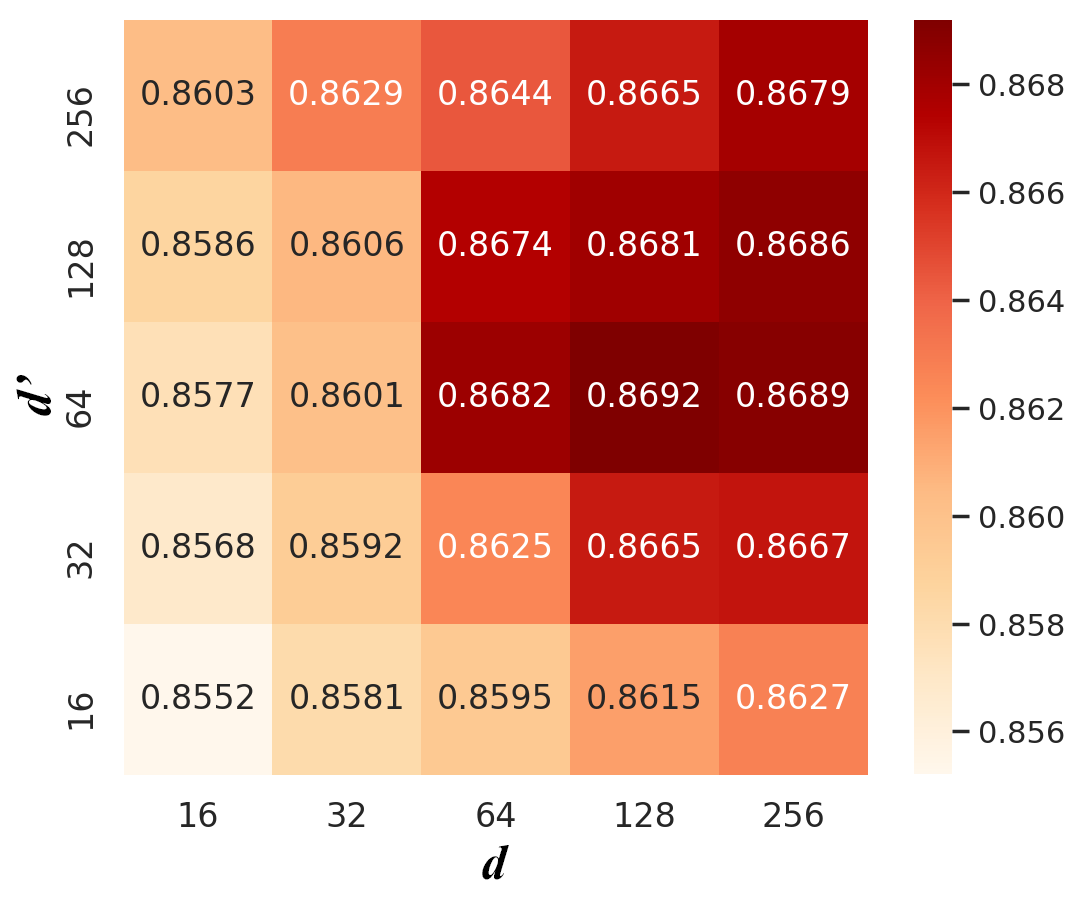
\includegraphics[width=0.30\linewidth]{res/hr_heatmap.png}}
% 	\quad 
	\subfigure[NDCG@10]{
		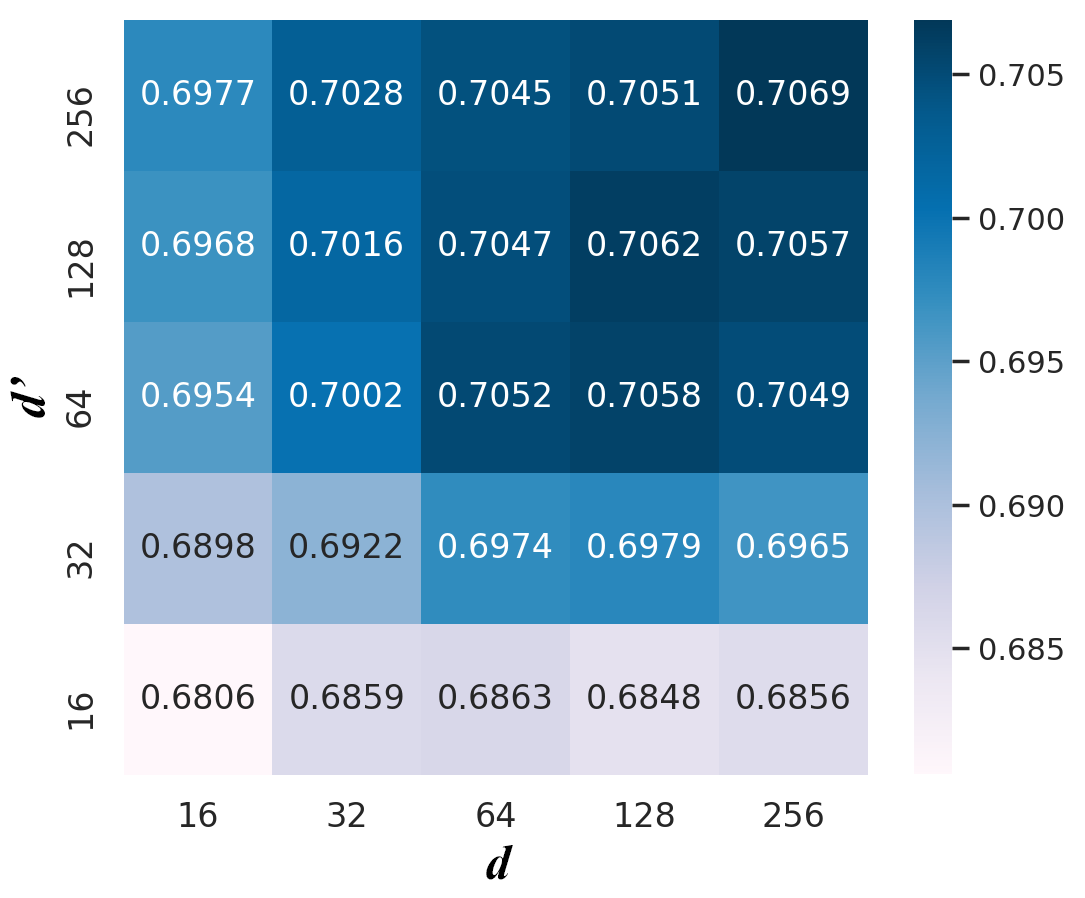
\includegraphics[width=0.30\linewidth]{res/ndcg_heatmap.png}}
	\caption{Top-10 recommendation Hit Ratio and NDCG scores w.r.t. various \# latent factor $d$ in BEM and $d'$ in KEM (\# layer = 4).}
	\label{fig:heatmap}
\end{figure}